\scanpage{132}
élément
\[
\operatorname{Tr}_{*}^{\unsure{*}}u\in A
\]
de telle façon que \inserted{$\alpha)$} si $L_\bullet$ est \uline{projectif} de type fini et à degrés bornés, alors
\[
\operatorname{Tr}_*u=\sum(-1)^i\operatorname{Tr}u_i,
\]
et $\beta)$ $\operatorname{Tr}_*u$ est ``stable par isomorphismes'' dans $D(A)$.

D'ailleurs, on peut aussi remplacer par l'ensemble des conditions

b) ``d'additivité'' pour un mapping cylindre

\figure{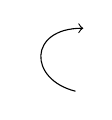
\begin{tikzpicture}\draw[->] (0,-.8)..controls(-.6,-.65) and(-.6,0)..(.1,0);\end{tikzpicture}}

a) Si $L_\bullet$ est réduit au degré $0$ et est libre, alors
\[
\operatorname{Tr}_*u=\operatorname{Tr}u
\]

\deleted{L'unicité} De plus, on \unsure{veut|vérifie} aussi d'autres propriétés formelles \unsure{utiles|usuelles}, signalons
\[
\text{c)}\quad\operatorname{Tr}uv=\operatorname{Tr}vu
\]
\[
\text{d)}\quad\operatorname{Tr}u\overset{\mathbb L}{\otimes}v=(\operatorname{Tr}u)(\operatorname{Tr}v)
\]
qui se ramènent aux formules correspondantes connues par ailleurs.

L'\uline{unicité} d'une fonction $\operatorname{Tr}_*$ satisfaisant aux conditions $\alpha)$ et $\beta)$ resp. a) et b) est claire. L'existence \deleted{\unsure{est}} se ramène à prouver que l'expression $\alpha)$ est
\mspage{131}
